
%%% Local Variables: 
%%% mode: latex
%%% TeX-master: t
%%% End: 

\usetikzlibrary{shapes}
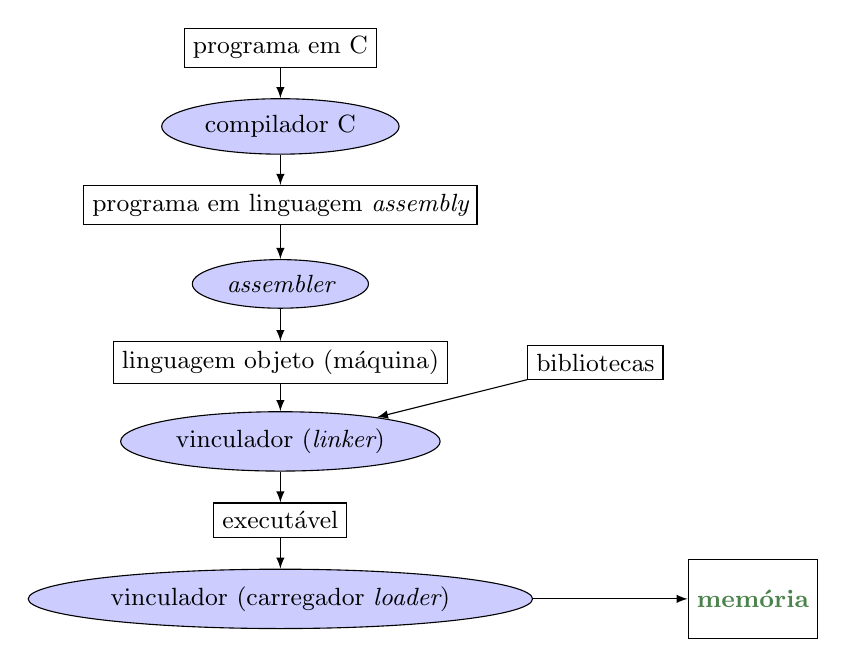
\begin{tikzpicture}[]
\small
  \node[rectangle,draw] (cprog) {programa em C};
  \node[fill=blue!20,ellipse,draw] (ccomp) [below of=cprog] {compilador C};
    \node[rectangle,draw] (sprog) [below of=ccomp] {programa em linguagem {\em
        assembly}};
    \node[fill=blue!20,ellipse,draw] (scomp) [below of=sprog] {{\em assembler}};
    \node[rectangle,draw] (mach) [below of=scomp] {linguagem objeto
      (máquina)};
    \node[rectangle,draw] (lib) [right of=mach,xshift=30mm] {bibliotecas};
    \node[fill=blue!20,ellipse,draw] (linker) [below of=mach] {vinculador ({\em linker})};
    \node[rectangle,draw] (exe) [below of=linker] {executável};
    \node[fill=blue!20,ellipse,draw] (loader) [below of=exe] {vinculador (carregador {\em
        loader})};
    \node[rectangle,minimum height=1cm,draw] (mem) [right of=loader,xshift=50mm] {\bf \color{green!30!black!70!}memória};
    
    \draw[->,>=latex] (cprog) -> (ccomp);
    \draw[->,>=latex] (ccomp) -> (sprog);
    \draw[->,>=latex] (sprog) -> (scomp);
    \draw[->,>=latex] (scomp) -> (mach);
    \draw[->,>=latex] (mach) -> (linker);
    \draw[->,>=latex] (lib) -> (linker);
    \draw[->,>=latex] (linker) -> (exe);
    \draw[->,>=latex]  (exe) -> (loader);
    \draw[->,>=latex] (loader) -> (mem);

\end{tikzpicture}